\documentclass[1p]{elsarticle_modified}
%\bibliographystyle{elsarticle-num}

%\usepackage[colorlinks]{hyperref}
%\usepackage{abbrmath_seonhwa} %\Abb, \Ascr, \Acal ,\Abf, \Afrak
\usepackage{amsfonts}
\usepackage{amssymb}
\usepackage{amsmath}
\usepackage{amsthm}
\usepackage{scalefnt}
\usepackage{amsbsy}
\usepackage{kotex}
\usepackage{caption}
\usepackage{subfig}
\usepackage{color}
\usepackage{graphicx}
\usepackage{xcolor} %% white, black, red, green, blue, cyan, magenta, yellow
\usepackage{float}
\usepackage{setspace}
\usepackage{hyperref}

\usepackage{tikz}
\usetikzlibrary{arrows}

\usepackage{multirow}
\usepackage{array} % fixed length table
\usepackage{hhline}

%%%%%%%%%%%%%%%%%%%%%
\makeatletter
\renewcommand*\env@matrix[1][\arraystretch]{%
	\edef\arraystretch{#1}%
	\hskip -\arraycolsep
	\let\@ifnextchar\new@ifnextchar
	\array{*\c@MaxMatrixCols c}}
\makeatother %https://tex.stackexchange.com/questions/14071/how-can-i-increase-the-line-spacing-in-a-matrix
%%%%%%%%%%%%%%%

\usepackage[normalem]{ulem}

\newcommand{\msout}[1]{\ifmmode\text{\sout{\ensuremath{#1}}}\else\sout{#1}\fi}
%SOURCE: \msout is \stkout macro in https://tex.stackexchange.com/questions/20609/strikeout-in-math-mode

\newcommand{\cancel}[1]{
	\ifmmode
	{\color{red}\msout{#1}}
	\else
	{\color{red}\sout{#1}}
	\fi
}

\newcommand{\add}[1]{
	{\color{blue}\uwave{#1}}
}

\newcommand{\replace}[2]{
	\ifmmode
	{\color{red}\msout{#1}}{\color{blue}\uwave{#2}}
	\else
	{\color{red}\sout{#1}}{\color{blue}\uwave{#2}}
	\fi
}

\newcommand{\Sol}{\mathcal{S}} %segment
\newcommand{\D}{D} %diagram
\newcommand{\A}{\mathcal{A}} %arc


%%%%%%%%%%%%%%%%%%%%%%%%%%%%%5 test

\def\sl{\operatorname{\textup{SL}}(2,\Cbb)}
\def\psl{\operatorname{\textup{PSL}}(2,\Cbb)}
\def\quan{\mkern 1mu \triangleright \mkern 1mu}

\theoremstyle{definition}
\newtheorem{thm}{Theorem}[section]
\newtheorem{prop}[thm]{Proposition}
\newtheorem{lem}[thm]{Lemma}
\newtheorem{ques}[thm]{Question}
\newtheorem{cor}[thm]{Corollary}
\newtheorem{defn}[thm]{Definition}
\newtheorem{exam}[thm]{Example}
\newtheorem{rmk}[thm]{Remark}
\newtheorem{alg}[thm]{Algorithm}

\newcommand{\I}{\sqrt{-1}}
\begin{document}

%\begin{frontmatter}
%
%\title{Boundary parabolic representations of knots up to 8 crossings}
%
%%% Group authors per affiliation:
%\author{Yunhi Cho} 
%\address{Department of Mathematics, University of Seoul, Seoul, Korea}
%\ead{yhcho@uos.ac.kr}
%
%
%\author{Seonhwa Kim} %\fnref{s_kim}}
%\address{Center for Geometry and Physics, Institute for Basic Science, Pohang, 37673, Korea}
%\ead{ryeona17@ibs.re.kr}
%
%\author{Hyuk Kim}
%\address{Department of Mathematical Sciences, Seoul National University, Seoul 08826, Korea}
%\ead{hyukkim@snu.ac.kr}
%
%\author{Seokbeom Yoon}
%\address{Department of Mathematical Sciences, Seoul National University, Seoul, 08826,  Korea}
%\ead{sbyoon15@snu.ac.kr}
%
%\begin{abstract}
%We find all boundary parabolic representation of knots up to 8 crossings.
%
%\end{abstract}
%\begin{keyword}
%    \MSC[2010] 57M25 
%\end{keyword}
%
%\end{frontmatter}

%\linenumbers
%\tableofcontents
%
\newcommand\colored[1]{\textcolor{white}{\rule[-0.35ex]{0.8em}{1.4ex}}\kern-0.8em\color{red} #1}%
%\newcommand\colored[1]{\textcolor{white}{ #1}\kern-2.17ex	\textcolor{white}{ #1}\kern-1.81ex	\textcolor{white}{ #1}\kern-2.15ex\color{red}#1	}

{\Large $\underline{12n_{0317}~(K12n_{0317})}$}

\setlength{\tabcolsep}{10pt}
\renewcommand{\arraystretch}{1.6}
\vspace{1cm}\begin{tabular}{m{100pt}>{\centering\arraybackslash}m{274pt}}
\multirow{5}{120pt}{
	\centering
	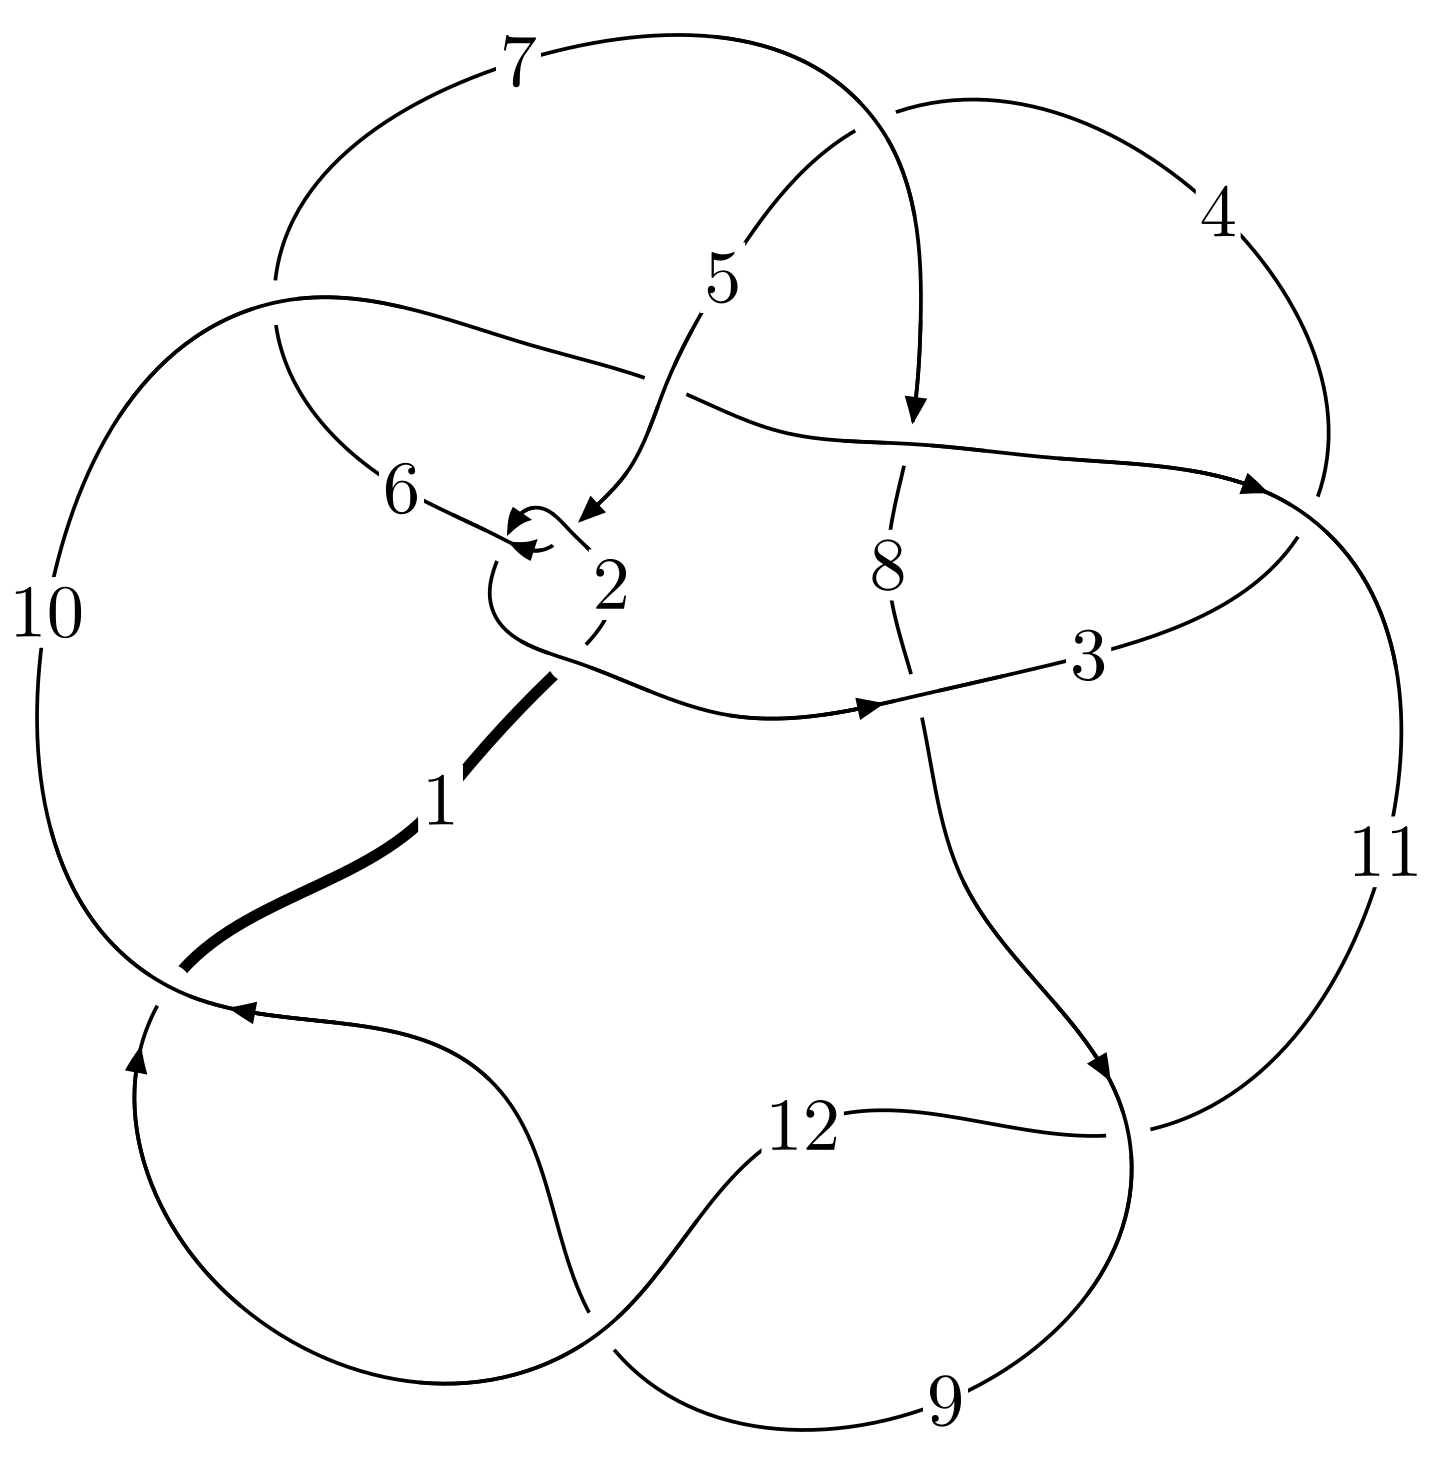
\includegraphics[width=112pt]{../../../GIT/diagram.site/Diagrams/png/2406_12n_0317.png}\\
\ \ \ A knot diagram\footnotemark}&
\allowdisplaybreaks
\textbf{Linearized knot diagam} \\
\cline{2-2}
 &
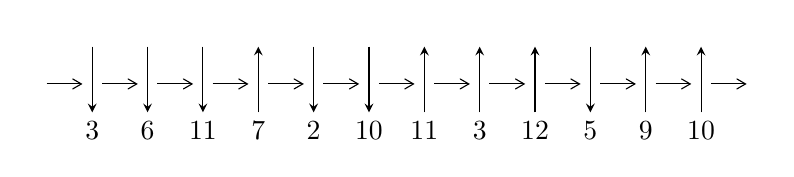
\begin{tikzpicture}[x=20pt, y=17pt]
	% nodes
	\node (C0) at (0, 0) {};
	\node (C1) at (1, 0) {};
	\node (C1U) at (1, +1) {};
	\node (C1D) at (1, -1) {3};

	\node (C2) at (2, 0) {};
	\node (C2U) at (2, +1) {};
	\node (C2D) at (2, -1) {6};

	\node (C3) at (3, 0) {};
	\node (C3U) at (3, +1) {};
	\node (C3D) at (3, -1) {11};

	\node (C4) at (4, 0) {};
	\node (C4U) at (4, +1) {};
	\node (C4D) at (4, -1) {7};

	\node (C5) at (5, 0) {};
	\node (C5U) at (5, +1) {};
	\node (C5D) at (5, -1) {2};

	\node (C6) at (6, 0) {};
	\node (C6U) at (6, +1) {};
	\node (C6D) at (6, -1) {10};

	\node (C7) at (7, 0) {};
	\node (C7U) at (7, +1) {};
	\node (C7D) at (7, -1) {11};

	\node (C8) at (8, 0) {};
	\node (C8U) at (8, +1) {};
	\node (C8D) at (8, -1) {3};

	\node (C9) at (9, 0) {};
	\node (C9U) at (9, +1) {};
	\node (C9D) at (9, -1) {12};

	\node (C10) at (10, 0) {};
	\node (C10U) at (10, +1) {};
	\node (C10D) at (10, -1) {5};

	\node (C11) at (11, 0) {};
	\node (C11U) at (11, +1) {};
	\node (C11D) at (11, -1) {9};

	\node (C12) at (12, 0) {};
	\node (C12U) at (12, +1) {};
	\node (C12D) at (12, -1) {10};
	\node (C13) at (13, 0) {};

	% arrows
	\draw[->,>={angle 60}]
	(C0) edge (C1) (C1) edge (C2) (C2) edge (C3) (C3) edge (C4) (C4) edge (C5) (C5) edge (C6) (C6) edge (C7) (C7) edge (C8) (C8) edge (C9) (C9) edge (C10) (C10) edge (C11) (C11) edge (C12) (C12) edge (C13) ;	\draw[->,>=stealth]
	(C1U) edge (C1D) (C2U) edge (C2D) (C3U) edge (C3D) (C4D) edge (C4U) (C5U) edge (C5D) (C6U) edge (C6D) (C7D) edge (C7U) (C8D) edge (C8U) (C9D) edge (C9U) (C10U) edge (C10D) (C11D) edge (C11U) (C12D) edge (C12U) ;
	\end{tikzpicture} \\
\hhline{~~} \\& 
\textbf{Solving Sequence} \\ \cline{2-2} 
 &
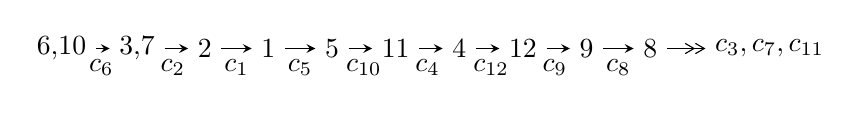
\begin{tikzpicture}[x=23pt, y=7pt]
	% node
	\node (A0) at (-1/8, 0) {6,10};
	\node (A1) at (17/16, 0) {3,7};
	\node (A2) at (17/8, 0) {2};
	\node (A3) at (25/8, 0) {1};
	\node (A4) at (33/8, 0) {5};
	\node (A5) at (41/8, 0) {11};
	\node (A6) at (49/8, 0) {4};
	\node (A7) at (57/8, 0) {12};
	\node (A8) at (65/8, 0) {9};
	\node (A9) at (73/8, 0) {8};
	\node (C1) at (1/2, -1) {$c_{6}$};
	\node (C2) at (13/8, -1) {$c_{2}$};
	\node (C3) at (21/8, -1) {$c_{1}$};
	\node (C4) at (29/8, -1) {$c_{5}$};
	\node (C5) at (37/8, -1) {$c_{10}$};
	\node (C6) at (45/8, -1) {$c_{4}$};
	\node (C7) at (53/8, -1) {$c_{12}$};
	\node (C8) at (61/8, -1) {$c_{9}$};
	\node (C9) at (69/8, -1) {$c_{8}$};
	\node (A10) at (11, 0) {$c_{3},c_{7},c_{11}$};

	% edge
	\draw[->,>=stealth]	
	(A0) edge (A1) (A1) edge (A2) (A2) edge (A3) (A3) edge (A4) (A4) edge (A5) (A5) edge (A6) (A6) edge (A7) (A7) edge (A8) (A8) edge (A9) ;
	\draw[->>,>={angle 60}]	
	(A9) edge (A10);
\end{tikzpicture} \\ 

\end{tabular} \\

\footnotetext{
The image of knot diagram is generated by the software ``\textbf{Draw programme}" developed by Andrew Bartholomew(\url{http://www.layer8.co.uk/maths/draw/index.htm\#Running-draw}), where we modified some parts for our purpose(\url{https://github.com/CATsTAILs/LinksPainter}).
}\phantom \\ \newline 
\centering \textbf{Ideals for irreducible components\footnotemark of $X_{\text{par}}$} 
 
\begin{align*}
I^u_{1}&=\langle 
1.91786\times10^{186} u^{49}-4.41920\times10^{186} u^{48}+\cdots+3.02291\times10^{188} b-8.34981\times10^{189},\\
\phantom{I^u_{1}}&\phantom{= \langle  }-8.33281\times10^{189} u^{49}+2.07014\times10^{190} u^{48}+\cdots+7.45751\times10^{191} a+3.95262\times10^{193},\\
\phantom{I^u_{1}}&\phantom{= \langle  }u^{50}-3 u^{49}+\cdots-20763 u+2467\rangle \\
I^u_{2}&=\langle 
-215 u^7+940 u^6-132 u^5-2470 u^4-1050 u^3-1010 u^2+714 b-1325 u+456,\\
\phantom{I^u_{2}}&\phantom{= \langle  }33 u^7-457 u^6+1280 u^5+678 u^4-3752 u^3-2070 u^2+714 a-1363 u-3697,\\
\phantom{I^u_{2}}&\phantom{= \langle  }u^8-4 u^7- u^6+12 u^5+8 u^4+6 u^3+11 u^2+2 u+1\rangle \\
\\
\end{align*}
\raggedright * 2 irreducible components of $\dim_{\mathbb{C}}=0$, with total 58 representations.\\
\footnotetext{All coefficients of polynomials are rational numbers. But the coefficients are sometimes approximated in decimal forms when there is not enough margin.}
\newpage
\renewcommand{\arraystretch}{1}
\centering \section*{I. $I^u_{1}= \langle 1.92\times10^{186} u^{49}-4.42\times10^{186} u^{48}+\cdots+3.02\times10^{188} b-8.35\times10^{189},\;-8.33\times10^{189} u^{49}+2.07\times10^{190} u^{48}+\cdots+7.46\times10^{191} a+3.95\times10^{193},\;u^{50}-3 u^{49}+\cdots-20763 u+2467 \rangle$}
\flushleft \textbf{(i) Arc colorings}\\
\begin{tabular}{m{7pt} m{180pt} m{7pt} m{180pt} }
\flushright $a_{6}=$&$\begin{pmatrix}1\\0\end{pmatrix}$ \\
\flushright $a_{10}=$&$\begin{pmatrix}0\\u\end{pmatrix}$ \\
\flushright $a_{3}=$&$\begin{pmatrix}0.0111737 u^{49}-0.0277592 u^{48}+\cdots+350.989 u-53.0019\\-0.00634441 u^{49}+0.0146190 u^{48}+\cdots-179.609 u+27.6218\end{pmatrix}$ \\
\flushright $a_{7}=$&$\begin{pmatrix}1\\u^2\end{pmatrix}$ \\
\flushright $a_{2}=$&$\begin{pmatrix}0.00482931 u^{49}-0.0131401 u^{48}+\cdots+171.380 u-25.3800\\-0.00634441 u^{49}+0.0146190 u^{48}+\cdots-179.609 u+27.6218\end{pmatrix}$ \\
\flushright $a_{1}=$&$\begin{pmatrix}-0.00125206 u^{49}+0.00578813 u^{48}+\cdots-123.642 u+25.1827\\-0.00103824 u^{49}+0.00521397 u^{48}+\cdots-175.306 u+29.1803\end{pmatrix}$ \\
\flushright $a_{5}=$&$\begin{pmatrix}0.00963656 u^{49}-0.0235349 u^{48}+\cdots+264.866 u-35.0739\\0.00325201 u^{49}-0.00880623 u^{48}+\cdots+84.8902 u-6.25925\end{pmatrix}$ \\
\flushright $a_{11}=$&$\begin{pmatrix}-0.0121639 u^{49}+0.0321646 u^{48}+\cdots-424.122 u+61.3195\\-0.000528690 u^{49}+0.00275946 u^{48}+\cdots-54.2826 u+5.53435\end{pmatrix}$ \\
\flushright $a_{4}=$&$\begin{pmatrix}0.00923043 u^{49}-0.0215045 u^{48}+\cdots+267.799 u-42.0742\\0.00540308 u^{49}-0.0125904 u^{48}+\cdots+102.752 u-8.26248\end{pmatrix}$ \\
\flushright $a_{12}=$&$\begin{pmatrix}-0.00125206 u^{49}+0.00578813 u^{48}+\cdots-123.642 u+25.1827\\0.00199645 u^{49}-0.000875897 u^{48}+\cdots-130.028 u+24.1675\end{pmatrix}$ \\
\flushright $a_{9}=$&$\begin{pmatrix}0.00315773 u^{49}-0.00845015 u^{48}+\cdots+155.251 u-29.5459\\0.00922550 u^{49}-0.0248174 u^{48}+\cdots+380.914 u-56.7451\end{pmatrix}$ \\
\flushright $a_{8}=$&$\begin{pmatrix}0.00526362 u^{49}-0.00912528 u^{48}+\cdots+65.8379 u-6.54803\\0.00917621 u^{49}-0.0232077 u^{48}+\cdots+309.861 u-48.3200\end{pmatrix}$\\&\end{tabular}
\flushleft \textbf{(ii) Obstruction class $= -1$}\\~\\
\flushleft \textbf{(iii) Cusp Shapes $= 0.0301306 u^{49}-0.0796043 u^{48}+\cdots+1263.65 u-235.993$}\\~\\
\newpage\renewcommand{\arraystretch}{1}
\flushleft \textbf{(iv) u-Polynomials at the component}\newline \\
\begin{tabular}{m{50pt}|m{274pt}}
Crossings & \hspace{64pt}u-Polynomials at each crossing \\
\hline $$\begin{aligned}c_{1}\end{aligned}$$&$\begin{aligned}
&u^{50}+27 u^{49}+\cdots+279 u+81
\end{aligned}$\\
\hline $$\begin{aligned}c_{2},c_{5}\end{aligned}$$&$\begin{aligned}
&u^{50}+3 u^{49}+\cdots+27 u+9
\end{aligned}$\\
\hline $$\begin{aligned}c_{3}\end{aligned}$$&$\begin{aligned}
&u^{50}-9 u^{49}+\cdots+6491 u+1543
\end{aligned}$\\
\hline $$\begin{aligned}c_{4},c_{8}\end{aligned}$$&$\begin{aligned}
&u^{50}+3 u^{49}+\cdots-72 u+36
\end{aligned}$\\
\hline $$\begin{aligned}c_{6}\end{aligned}$$&$\begin{aligned}
&u^{50}+3 u^{49}+\cdots+20763 u+2467
\end{aligned}$\\
\hline $$\begin{aligned}c_{7}\end{aligned}$$&$\begin{aligned}
&u^{50}-3 u^{49}+\cdots-1360 u+64
\end{aligned}$\\
\hline $$\begin{aligned}c_{9},c_{11},c_{12}\end{aligned}$$&$\begin{aligned}
&u^{50}+5 u^{49}+\cdots+11 u+1
\end{aligned}$\\
\hline $$\begin{aligned}c_{10}\end{aligned}$$&$\begin{aligned}
&u^{50}- u^{49}+\cdots+3 u+1
\end{aligned}$\\
\hline
\end{tabular}\\~\\
\newpage\renewcommand{\arraystretch}{1}
\flushleft \textbf{(v) Riley Polynomials at the component}\newline \\
\begin{tabular}{m{50pt}|m{274pt}}
Crossings & \hspace{64pt}Riley Polynomials at each crossing \\
\hline $$\begin{aligned}c_{1}\end{aligned}$$&$\begin{aligned}
&y^{50}-3 y^{49}+\cdots-40743 y+6561
\end{aligned}$\\
\hline $$\begin{aligned}c_{2},c_{5}\end{aligned}$$&$\begin{aligned}
&y^{50}-27 y^{49}+\cdots-279 y+81
\end{aligned}$\\
\hline $$\begin{aligned}c_{3}\end{aligned}$$&$\begin{aligned}
&y^{50}-137 y^{49}+\cdots+71302107 y+2380849
\end{aligned}$\\
\hline $$\begin{aligned}c_{4},c_{8}\end{aligned}$$&$\begin{aligned}
&y^{50}+53 y^{49}+\cdots+2232 y+1296
\end{aligned}$\\
\hline $$\begin{aligned}c_{6}\end{aligned}$$&$\begin{aligned}
&y^{50}+43 y^{49}+\cdots-163462273 y+6086089
\end{aligned}$\\
\hline $$\begin{aligned}c_{7}\end{aligned}$$&$\begin{aligned}
&y^{50}+143 y^{49}+\cdots+1959168 y+4096
\end{aligned}$\\
\hline $$\begin{aligned}c_{9},c_{11},c_{12}\end{aligned}$$&$\begin{aligned}
&y^{50}-39 y^{49}+\cdots-35 y+1
\end{aligned}$\\
\hline $$\begin{aligned}c_{10}\end{aligned}$$&$\begin{aligned}
&y^{50}+9 y^{49}+\cdots-35 y+1
\end{aligned}$\\
\hline
\end{tabular}\\~\\
\newpage\flushleft \textbf{(vi) Complex Volumes and Cusp Shapes}
$$\begin{array}{c|c|c}  
\text{Solutions to }I^u_{1}& \I (\text{vol} + \sqrt{-1}CS) & \text{Cusp shape}\\
 \hline 
\begin{aligned}
u &= -0.663546 + 0.807023 I \\
a &= -0.149925 - 1.093180 I \\
b &= \phantom{-}0.227624 + 0.962311 I\end{aligned}
 & \phantom{-}3.78569 + 3.81617 I & \phantom{-}5.99930 - 6.58404 I \\ \hline\begin{aligned}
u &= -0.663546 - 0.807023 I \\
a &= -0.149925 + 1.093180 I \\
b &= \phantom{-}0.227624 - 0.962311 I\end{aligned}
 & \phantom{-}3.78569 - 3.81617 I & \phantom{-}5.99930 + 6.58404 I \\ \hline\begin{aligned}
u &= \phantom{-}0.989845 + 0.334652 I \\
a &= -0.852002 - 0.574478 I \\
b &= \phantom{-}0.075144 + 0.777118 I\end{aligned}
 & -2.75103 + 1.66476 I & \phantom{-0.000000 } 0 \\ \hline\begin{aligned}
u &= \phantom{-}0.989845 - 0.334652 I \\
a &= -0.852002 + 0.574478 I \\
b &= \phantom{-}0.075144 - 0.777118 I\end{aligned}
 & -2.75103 - 1.66476 I & \phantom{-0.000000 } 0 \\ \hline\begin{aligned}
u &= -1.038610 + 0.115738 I \\
a &= \phantom{-}0.07663 + 1.46376 I \\
b &= \phantom{-}1.283560 - 0.355028 I\end{aligned}
 & -11.43970 + 0.61215 I & -5.56930 - 0.95685 I \\ \hline\begin{aligned}
u &= -1.038610 - 0.115738 I \\
a &= \phantom{-}0.07663 - 1.46376 I \\
b &= \phantom{-}1.283560 + 0.355028 I\end{aligned}
 & -11.43970 - 0.61215 I & -5.56930 + 0.95685 I \\ \hline\begin{aligned}
u &= -0.976418 + 0.409184 I \\
a &= -0.117550 - 1.213630 I \\
b &= -0.889554 - 0.262388 I\end{aligned}
 & \phantom{-}6.22845 - 1.17042 I & -3.22256 + 0. I\phantom{ +0.000000I} \\ \hline\begin{aligned}
u &= -0.976418 - 0.409184 I \\
a &= -0.117550 + 1.213630 I \\
b &= -0.889554 + 0.262388 I\end{aligned}
 & \phantom{-}6.22845 + 1.17042 I & -3.22256 + 0. I\phantom{ +0.000000I} \\ \hline\begin{aligned}
u &= \phantom{-}0.856388 + 0.349802 I \\
a &= -0.217606 - 1.026260 I \\
b &= -0.931404 + 0.588464 I\end{aligned}
 & -1.84212 + 2.10652 I & -6.74335 - 2.91333 I \\ \hline\begin{aligned}
u &= \phantom{-}0.856388 - 0.349802 I \\
a &= -0.217606 + 1.026260 I \\
b &= -0.931404 - 0.588464 I\end{aligned}
 & -1.84212 - 2.10652 I & -6.74335 + 2.91333 I\\
 \hline 
 \end{array}$$\newpage$$\begin{array}{c|c|c}  
\text{Solutions to }I^u_{1}& \I (\text{vol} + \sqrt{-1}CS) & \text{Cusp shape}\\
 \hline 
\begin{aligned}
u &= -0.666952 + 0.913096 I \\
a &= -0.008649 - 0.157261 I \\
b &= \phantom{-}0.697921 + 0.367007 I\end{aligned}
 & \phantom{-}1.14279 - 1.51204 I & \phantom{-0.000000 } 0 \\ \hline\begin{aligned}
u &= -0.666952 - 0.913096 I \\
a &= -0.008649 + 0.157261 I \\
b &= \phantom{-}0.697921 - 0.367007 I\end{aligned}
 & \phantom{-}1.14279 + 1.51204 I & \phantom{-0.000000 } 0 \\ \hline\begin{aligned}
u &= \phantom{-}0.553985 + 0.646141 I \\
a &= \phantom{-}0.195853 + 0.760473 I \\
b &= \phantom{-}0.095352 - 0.510935 I\end{aligned}
 & \phantom{-}0.078263 - 1.314770 I & \phantom{-}0.82809 + 5.18119 I \\ \hline\begin{aligned}
u &= \phantom{-}0.553985 - 0.646141 I \\
a &= \phantom{-}0.195853 - 0.760473 I \\
b &= \phantom{-}0.095352 + 0.510935 I\end{aligned}
 & \phantom{-}0.078263 + 1.314770 I & \phantom{-}0.82809 - 5.18119 I \\ \hline\begin{aligned}
u &= \phantom{-}0.772929 + 0.314148 I \\
a &= -0.24097 - 2.31460 I \\
b &= \phantom{-}1.197270 + 0.484749 I\end{aligned}
 & -6.02259 - 6.28550 I & -2.35130 + 4.21184 I \\ \hline\begin{aligned}
u &= \phantom{-}0.772929 - 0.314148 I \\
a &= -0.24097 + 2.31460 I \\
b &= \phantom{-}1.197270 - 0.484749 I\end{aligned}
 & -6.02259 + 6.28550 I & -2.35130 - 4.21184 I \\ \hline\begin{aligned}
u &= \phantom{-}1.232170 + 0.182436 I \\
a &= \phantom{-}0.142577 + 0.722468 I \\
b &= \phantom{-}1.327810 - 0.185520 I\end{aligned}
 & -8.47541 - 5.36250 I & \phantom{-0.000000 } 0 \\ \hline\begin{aligned}
u &= \phantom{-}1.232170 - 0.182436 I \\
a &= \phantom{-}0.142577 - 0.722468 I \\
b &= \phantom{-}1.327810 + 0.185520 I\end{aligned}
 & -8.47541 + 5.36250 I & \phantom{-0.000000 } 0 \\ \hline\begin{aligned}
u &= -0.665058 + 0.099931 I \\
a &= -0.450338 - 0.389982 I \\
b &= -1.190510 + 0.112073 I\end{aligned}
 & -1.93432 + 0.03774 I & -6.75026 + 1.46726 I \\ \hline\begin{aligned}
u &= -0.665058 - 0.099931 I \\
a &= -0.450338 + 0.389982 I \\
b &= -1.190510 - 0.112073 I\end{aligned}
 & -1.93432 - 0.03774 I & -6.75026 - 1.46726 I\\
 \hline 
 \end{array}$$\newpage$$\begin{array}{c|c|c}  
\text{Solutions to }I^u_{1}& \I (\text{vol} + \sqrt{-1}CS) & \text{Cusp shape}\\
 \hline 
\begin{aligned}
u &= -1.219730 + 0.587243 I \\
a &= -0.224495 + 0.844921 I \\
b &= -0.158932 - 0.906350 I\end{aligned}
 & -6.85044 + 3.69371 I & \phantom{-0.000000 } 0 \\ \hline\begin{aligned}
u &= -1.219730 - 0.587243 I \\
a &= -0.224495 - 0.844921 I \\
b &= -0.158932 + 0.906350 I\end{aligned}
 & -6.85044 - 3.69371 I & \phantom{-0.000000 } 0 \\ \hline\begin{aligned}
u &= \phantom{-}0.572239 + 0.270156 I \\
a &= \phantom{-}0.04237 + 1.45670 I \\
b &= -1.203320 - 0.645182 I\end{aligned}
 & -1.68209 - 2.49103 I & -8.75436 + 6.26567 I \\ \hline\begin{aligned}
u &= \phantom{-}0.572239 - 0.270156 I \\
a &= \phantom{-}0.04237 - 1.45670 I \\
b &= -1.203320 + 0.645182 I\end{aligned}
 & -1.68209 + 2.49103 I & -8.75436 - 6.26567 I \\ \hline\begin{aligned}
u &= -0.504003 + 0.379964 I \\
a &= \phantom{-}1.17363 + 1.99927 I \\
b &= -0.391480 - 0.395210 I\end{aligned}
 & \phantom{-}2.40372 + 0.20646 I & \phantom{-}4.09834 + 1.60523 I \\ \hline\begin{aligned}
u &= -0.504003 - 0.379964 I \\
a &= \phantom{-}1.17363 - 1.99927 I \\
b &= -0.391480 + 0.395210 I\end{aligned}
 & \phantom{-}2.40372 - 0.20646 I & \phantom{-}4.09834 - 1.60523 I \\ \hline\begin{aligned}
u &= \phantom{-}0.988631 + 0.981714 I \\
a &= \phantom{-}0.270126 + 0.926267 I \\
b &= -0.867195 - 0.191758 I\end{aligned}
 & -1.69134 - 0.97922 I & \phantom{-0.000000 } 0 \\ \hline\begin{aligned}
u &= \phantom{-}0.988631 - 0.981714 I \\
a &= \phantom{-}0.270126 - 0.926267 I \\
b &= -0.867195 + 0.191758 I\end{aligned}
 & -1.69134 + 0.97922 I & \phantom{-0.000000 } 0 \\ \hline\begin{aligned}
u &= -0.74624 + 1.31133 I \\
a &= \phantom{-}0.534856 - 1.257750 I \\
b &= -1.029620 + 0.449989 I\end{aligned}
 & \phantom{-}0.61177 + 3.94770 I & \phantom{-0.000000 } 0 \\ \hline\begin{aligned}
u &= -0.74624 - 1.31133 I \\
a &= \phantom{-}0.534856 + 1.257750 I \\
b &= -1.029620 - 0.449989 I\end{aligned}
 & \phantom{-}0.61177 - 3.94770 I & \phantom{-0.000000 } 0\\
 \hline 
 \end{array}$$\newpage$$\begin{array}{c|c|c}  
\text{Solutions to }I^u_{1}& \I (\text{vol} + \sqrt{-1}CS) & \text{Cusp shape}\\
 \hline 
\begin{aligned}
u &= -1.08135 + 1.05259 I \\
a &= -0.017301 + 1.142600 I \\
b &= \phantom{-}1.215370 - 0.580128 I\end{aligned}
 & \phantom{-}0.77226 + 9.34517 I & \phantom{-0.000000 } 0 \\ \hline\begin{aligned}
u &= -1.08135 - 1.05259 I \\
a &= -0.017301 - 1.142600 I \\
b &= \phantom{-}1.215370 + 0.580128 I\end{aligned}
 & \phantom{-}0.77226 - 9.34517 I & \phantom{-0.000000 } 0 \\ \hline\begin{aligned}
u &= \phantom{-}0.345794 + 0.327250 I \\
a &= -0.38006 - 1.82618 I \\
b &= \phantom{-}0.824382 - 0.600279 I\end{aligned}
 & \phantom{-}8.49427 + 2.35863 I & \phantom{-}9.67846 - 4.20278 I \\ \hline\begin{aligned}
u &= \phantom{-}0.345794 - 0.327250 I \\
a &= -0.38006 + 1.82618 I \\
b &= \phantom{-}0.824382 + 0.600279 I\end{aligned}
 & \phantom{-}8.49427 - 2.35863 I & \phantom{-}9.67846 + 4.20278 I \\ \hline\begin{aligned}
u &= \phantom{-}1.29112 + 0.85257 I \\
a &= \phantom{-}0.129364 - 0.986571 I \\
b &= -0.333303 + 0.969379 I\end{aligned}
 & -2.65959 - 9.10689 I & \phantom{-0.000000 } 0 \\ \hline\begin{aligned}
u &= \phantom{-}1.29112 - 0.85257 I \\
a &= \phantom{-}0.129364 + 0.986571 I \\
b &= -0.333303 - 0.969379 I\end{aligned}
 & -2.65959 + 9.10689 I & \phantom{-0.000000 } 0 \\ \hline\begin{aligned}
u &= \phantom{-}1.27077 + 0.89539 I \\
a &= \phantom{-}0.166830 - 0.847725 I \\
b &= \phantom{-}1.141690 + 0.428927 I\end{aligned}
 & -2.80920 - 5.12014 I & \phantom{-0.000000 } 0 \\ \hline\begin{aligned}
u &= \phantom{-}1.27077 - 0.89539 I \\
a &= \phantom{-}0.166830 + 0.847725 I \\
b &= \phantom{-}1.141690 - 0.428927 I\end{aligned}
 & -2.80920 + 5.12014 I & \phantom{-0.000000 } 0 \\ \hline\begin{aligned}
u &= \phantom{-}0.353111 + 0.190645 I \\
a &= \phantom{-}1.170400 + 0.676061 I \\
b &= -0.715685 - 0.985730 I\end{aligned}
 & \phantom{-}0.02992 - 4.02059 I & -0.43876 + 11.60977 I \\ \hline\begin{aligned}
u &= \phantom{-}0.353111 - 0.190645 I \\
a &= \phantom{-}1.170400 - 0.676061 I \\
b &= -0.715685 + 0.985730 I\end{aligned}
 & \phantom{-}0.02992 + 4.02059 I & -0.43876 - 11.60977 I\\
 \hline 
 \end{array}$$\newpage$$\begin{array}{c|c|c}  
\text{Solutions to }I^u_{1}& \I (\text{vol} + \sqrt{-1}CS) & \text{Cusp shape}\\
 \hline 
\begin{aligned}
u &= \phantom{-}1.68410 + 0.25011 I \\
a &= -0.209855 + 0.322284 I \\
b &= -1.203160 - 0.421900 I\end{aligned}
 & -6.47293 - 2.51617 I & \phantom{-0.000000 } 0 \\ \hline\begin{aligned}
u &= \phantom{-}1.68410 - 0.25011 I \\
a &= -0.209855 - 0.322284 I \\
b &= -1.203160 + 0.421900 I\end{aligned}
 & -6.47293 + 2.51617 I & \phantom{-0.000000 } 0 \\ \hline\begin{aligned}
u &= -1.75503 + 0.68133 I \\
a &= -0.093305 - 0.780362 I \\
b &= -1.229330 + 0.542511 I\end{aligned}
 & -10.09350 + 8.94227 I & \phantom{-0.000000 } 0 \\ \hline\begin{aligned}
u &= -1.75503 - 0.68133 I \\
a &= -0.093305 + 0.780362 I \\
b &= -1.229330 - 0.542511 I\end{aligned}
 & -10.09350 - 8.94227 I & \phantom{-0.000000 } 0 \\ \hline\begin{aligned}
u &= \phantom{-}1.64933 + 1.01561 I \\
a &= -0.043620 + 1.103240 I \\
b &= -1.205270 - 0.631705 I\end{aligned}
 & -5.3380 - 14.9199 I & \phantom{-0.000000 } 0 \\ \hline\begin{aligned}
u &= \phantom{-}1.64933 - 1.01561 I \\
a &= -0.043620 - 1.103240 I \\
b &= -1.205270 + 0.631705 I\end{aligned}
 & -5.3380 + 14.9199 I & \phantom{-0.000000 } 0 \\ \hline\begin{aligned}
u &= -2.11053 + 0.20467 I \\
a &= \phantom{-}0.206325 + 0.667266 I \\
b &= \phantom{-}0.947425 - 0.426776 I\end{aligned}
 & \phantom{-}0.37870 + 1.85992 I & \phantom{-0.000000 } 0 \\ \hline\begin{aligned}
u &= -2.11053 - 0.20467 I \\
a &= \phantom{-}0.206325 - 0.667266 I \\
b &= \phantom{-}0.947425 + 0.426776 I\end{aligned}
 & \phantom{-}0.37870 - 1.85992 I & \phantom{-0.000000 } 0 \\ \hline\begin{aligned}
u &= \phantom{-}0.36706 + 6.35882 I \\
a &= \phantom{-}0.047914 + 1.066360 I \\
b &= \phantom{-}0.815200 - 0.491841 I\end{aligned}
 & \phantom{-}0.07826 + 2.04862 I & \phantom{-0.000000 } 0 \\ \hline\begin{aligned}
u &= \phantom{-}0.36706 - 6.35882 I \\
a &= \phantom{-}0.047914 - 1.066360 I \\
b &= \phantom{-}0.815200 + 0.491841 I\end{aligned}
 & \phantom{-}0.07826 - 2.04862 I & \phantom{-0.000000 } 0\\
 \hline 
 \end{array}$$\newpage\newpage\renewcommand{\arraystretch}{1}
\centering \section*{II. $I^u_{2}= \langle -215 u^7+940 u^6+\cdots+714 b+456,\;33 u^7-457 u^6+\cdots+714 a-3697,\;u^8-4 u^7+\cdots+2 u+1 \rangle$}
\flushleft \textbf{(i) Arc colorings}\\
\begin{tabular}{m{7pt} m{180pt} m{7pt} m{180pt} }
\flushright $a_{6}=$&$\begin{pmatrix}1\\0\end{pmatrix}$ \\
\flushright $a_{10}=$&$\begin{pmatrix}0\\u\end{pmatrix}$ \\
\flushright $a_{3}=$&$\begin{pmatrix}-0.0462185 u^{7}+0.640056 u^{6}+\cdots+1.90896 u+5.17787\\0.301120 u^{7}-1.31653 u^{6}+\cdots+1.85574 u-0.638655\end{pmatrix}$ \\
\flushright $a_{7}=$&$\begin{pmatrix}1\\u^2\end{pmatrix}$ \\
\flushright $a_{2}=$&$\begin{pmatrix}0.254902 u^{7}-0.676471 u^{6}+\cdots+3.76471 u+4.53922\\0.301120 u^{7}-1.31653 u^{6}+\cdots+1.85574 u-0.638655\end{pmatrix}$ \\
\flushright $a_{1}=$&$\begin{pmatrix}1.79552 u^{7}-7.23389 u^{6}+\cdots+17.5770 u+3.05462\\-0.151261 u^{7}+0.564426 u^{6}+\cdots-1.69188 u-0.948179\end{pmatrix}$ \\
\flushright $a_{5}=$&$\begin{pmatrix}-0.610644 u^{7}+3.00700 u^{6}+\cdots-3.87955 u+4.56723\\0.343137 u^{7}-1.35294 u^{6}+\cdots+3.02941 u-0.254902\end{pmatrix}$ \\
\flushright $a_{11}=$&$\begin{pmatrix}-2.79552 u^{7}+11.2339 u^{6}+\cdots-28.5770 u-5.05462\\0.203081 u^{7}-0.620448 u^{6}+\cdots+4.22829 u+1.74370\end{pmatrix}$ \\
\flushright $a_{4}=$&$\begin{pmatrix}-1.06303 u^{7}+4.88796 u^{6}+\cdots-7.42717 u+4.25770\\0.366947 u^{7}-1.32913 u^{6}+\cdots+3.33894 u-0.326331\end{pmatrix}$ \\
\flushright $a_{12}=$&$\begin{pmatrix}1.79552 u^{7}-7.23389 u^{6}+\cdots+17.5770 u+3.05462\\-0.302521 u^{7}+1.12885 u^{6}+\cdots-3.38375 u-0.896359\end{pmatrix}$ \\
\flushright $a_{9}=$&$\begin{pmatrix}2.79552 u^{7}-11.2339 u^{6}+\cdots+28.5770 u+5.05462\\-0.354342 u^{7}+1.18487 u^{6}+\cdots-4.92017 u-1.69188\end{pmatrix}$ \\
\flushright $a_{8}=$&$\begin{pmatrix}4.53922 u^{7}-18.4118 u^{6}+\cdots+45.6176 u+6.31373\\-0.697479 u^{7}+2.53782 u^{6}+\cdots-7.94958 u-2.43697\end{pmatrix}$\\&\end{tabular}
\flushleft \textbf{(ii) Obstruction class $= 1$}\\~\\
\flushleft \textbf{(iii) Cusp Shapes $= -\frac{70}{51} u^7+\frac{92}{17} u^6+\frac{112}{51} u^5-\frac{956}{51} u^4-\frac{568}{51} u^3-\frac{196}{51} u^2-\frac{206}{17} u+\frac{52}{51}$}\\~\\
\newpage\renewcommand{\arraystretch}{1}
\flushleft \textbf{(iv) u-Polynomials at the component}\newline \\
\begin{tabular}{m{50pt}|m{274pt}}
Crossings & \hspace{64pt}u-Polynomials at each crossing \\
\hline $$\begin{aligned}c_{1}\end{aligned}$$&$\begin{aligned}
&(u^2- u+1)^4
\end{aligned}$\\
\hline $$\begin{aligned}c_{2},c_{5}\end{aligned}$$&$\begin{aligned}
&(u^4- u^2+1)^2
\end{aligned}$\\
\hline $$\begin{aligned}c_{3}\end{aligned}$$&$\begin{aligned}
&u^8+2 u^7+11 u^6+6 u^5+8 u^4+12 u^3- u^2-4 u+1
\end{aligned}$\\
\hline $$\begin{aligned}c_{4},c_{8}\end{aligned}$$&$\begin{aligned}
&(u^2+1)^4
\end{aligned}$\\
\hline $$\begin{aligned}c_{6}\end{aligned}$$&$\begin{aligned}
&u^8-4 u^7- u^6+12 u^5+8 u^4+6 u^3+11 u^2+2 u+1
\end{aligned}$\\
\hline $$\begin{aligned}c_{7}\end{aligned}$$&$\begin{aligned}
&u^8-8 u^7+25 u^6-38 u^5+33 u^4-28 u^3+28 u^2-16 u+4
\end{aligned}$\\
\hline $$\begin{aligned}c_{9}\end{aligned}$$&$\begin{aligned}
&(u^2- u-1)^4
\end{aligned}$\\
\hline $$\begin{aligned}c_{10}\end{aligned}$$&$\begin{aligned}
&(u^4+3 u^2+1)^2
\end{aligned}$\\
\hline $$\begin{aligned}c_{11},c_{12}\end{aligned}$$&$\begin{aligned}
&(u^2+u-1)^4
\end{aligned}$\\
\hline
\end{tabular}\\~\\
\newpage\renewcommand{\arraystretch}{1}
\flushleft \textbf{(v) Riley Polynomials at the component}\newline \\
\begin{tabular}{m{50pt}|m{274pt}}
Crossings & \hspace{64pt}Riley Polynomials at each crossing \\
\hline $$\begin{aligned}c_{1}\end{aligned}$$&$\begin{aligned}
&(y^2+y+1)^4
\end{aligned}$\\
\hline $$\begin{aligned}c_{2},c_{5}\end{aligned}$$&$\begin{aligned}
&(y^2- y+1)^4
\end{aligned}$\\
\hline $$\begin{aligned}c_{3}\end{aligned}$$&$\begin{aligned}
&y^8+18 y^7+113 y^6+90 y^5-84 y^4-90 y^3+113 y^2-18 y+1
\end{aligned}$\\
\hline $$\begin{aligned}c_{4},c_{8}\end{aligned}$$&$\begin{aligned}
&(y+1)^8
\end{aligned}$\\
\hline $$\begin{aligned}c_{6}\end{aligned}$$&$\begin{aligned}
&y^8-18 y^7+113 y^6-90 y^5-84 y^4+90 y^3+113 y^2+18 y+1
\end{aligned}$\\
\hline $$\begin{aligned}c_{7}\end{aligned}$$&$\begin{aligned}
&y^8-14 y^7+83 y^6-186 y^5+113 y^4+48 y^3+152 y^2-32 y+16
\end{aligned}$\\
\hline $$\begin{aligned}c_{9},c_{11},c_{12}\end{aligned}$$&$\begin{aligned}
&(y^2-3 y+1)^4
\end{aligned}$\\
\hline $$\begin{aligned}c_{10}\end{aligned}$$&$\begin{aligned}
&(y^2+3 y+1)^4
\end{aligned}$\\
\hline
\end{tabular}\\~\\
\newpage\flushleft \textbf{(vi) Complex Volumes and Cusp Shapes}
$$\begin{array}{c|c|c}  
\text{Solutions to }I^u_{2}& \I (\text{vol} + \sqrt{-1}CS) & \text{Cusp shape}\\
 \hline 
\begin{aligned}
u &= \phantom{-}0.216775 + 0.809017 I \\
a &= \phantom{-}0.712758 + 0.809017 I \\
b &= -0.866025 - 0.500000 I\end{aligned}
 & -0.65797 - 2.02988 I & \phantom{-}2.00000 + 3.46410 I \\ \hline\begin{aligned}
u &= \phantom{-}0.216775 - 0.809017 I \\
a &= \phantom{-}0.712758 - 0.809017 I \\
b &= -0.866025 + 0.500000 I\end{aligned}
 & -0.65797 + 2.02988 I & \phantom{-}2.00000 - 3.46410 I \\ \hline\begin{aligned}
u &= -1.153270 + 0.309017 I \\
a &= \phantom{-}0.350750 + 0.309017 I \\
b &= \phantom{-}0.866025 + 0.500000 I\end{aligned}
 & \phantom{-}7.23771 - 2.02988 I & \phantom{-}2.00000 + 3.46410 I \\ \hline\begin{aligned}
u &= -1.153270 - 0.309017 I \\
a &= \phantom{-}0.350750 - 0.309017 I \\
b &= \phantom{-}0.866025 - 0.500000 I\end{aligned}
 & \phantom{-}7.23771 + 2.02988 I & \phantom{-}2.00000 - 3.46410 I \\ \hline\begin{aligned}
u &= -0.082801 + 0.309017 I \\
a &= \phantom{-}4.88532 + 0.30902 I \\
b &= -0.866025 + 0.500000 I\end{aligned}
 & \phantom{-}7.23771 + 2.02988 I & \phantom{-}2.00000 - 3.46410 I \\ \hline\begin{aligned}
u &= -0.082801 - 0.309017 I \\
a &= \phantom{-}4.88532 - 0.30902 I \\
b &= -0.866025 - 0.500000 I\end{aligned}
 & \phantom{-}7.23771 - 2.02988 I & \phantom{-}2.00000 + 3.46410 I \\ \hline\begin{aligned}
u &= \phantom{-}3.01929 + 0.80902 I \\
a &= \phantom{-}0.051174 + 0.809017 I \\
b &= \phantom{-}0.866025 - 0.500000 I\end{aligned}
 & -0.65797 + 2.02988 I & \phantom{-}2.00000 - 3.46410 I \\ \hline\begin{aligned}
u &= \phantom{-}3.01929 - 0.80902 I \\
a &= \phantom{-}0.051174 - 0.809017 I \\
b &= \phantom{-}0.866025 + 0.500000 I\end{aligned}
 & -0.65797 - 2.02988 I & \phantom{-}2.00000 + 3.46410 I\\
 \hline 
 \end{array}$$\newpage
\newpage\renewcommand{\arraystretch}{1}
\centering \section*{ III. u-Polynomials}
\begin{tabular}{m{50pt}|m{274pt}}
Crossings & \hspace{64pt}u-Polynomials at each crossing \\
\hline $$\begin{aligned}c_{1}\end{aligned}$$&$\begin{aligned}
&((u^2- u+1)^4)(u^{50}+27 u^{49}+\cdots+279 u+81)
\end{aligned}$\\
\hline $$\begin{aligned}c_{2},c_{5}\end{aligned}$$&$\begin{aligned}
&((u^4- u^2+1)^2)(u^{50}+3 u^{49}+\cdots+27 u+9)
\end{aligned}$\\
\hline $$\begin{aligned}c_{3}\end{aligned}$$&$\begin{aligned}
&(u^8+2 u^7+11 u^6+6 u^5+8 u^4+12 u^3- u^2-4 u+1)\\
&\cdot(u^{50}-9 u^{49}+\cdots+6491 u+1543)
\end{aligned}$\\
\hline $$\begin{aligned}c_{4},c_{8}\end{aligned}$$&$\begin{aligned}
&((u^2+1)^4)(u^{50}+3 u^{49}+\cdots-72 u+36)
\end{aligned}$\\
\hline $$\begin{aligned}c_{6}\end{aligned}$$&$\begin{aligned}
&(u^8-4 u^7- u^6+12 u^5+8 u^4+6 u^3+11 u^2+2 u+1)\\
&\cdot(u^{50}+3 u^{49}+\cdots+20763 u+2467)
\end{aligned}$\\
\hline $$\begin{aligned}c_{7}\end{aligned}$$&$\begin{aligned}
&(u^8-8 u^7+25 u^6-38 u^5+33 u^4-28 u^3+28 u^2-16 u+4)\\
&\cdot(u^{50}-3 u^{49}+\cdots-1360 u+64)
\end{aligned}$\\
\hline $$\begin{aligned}c_{9}\end{aligned}$$&$\begin{aligned}
&((u^2- u-1)^4)(u^{50}+5 u^{49}+\cdots+11 u+1)
\end{aligned}$\\
\hline $$\begin{aligned}c_{10}\end{aligned}$$&$\begin{aligned}
&((u^4+3 u^2+1)^2)(u^{50}- u^{49}+\cdots+3 u+1)
\end{aligned}$\\
\hline $$\begin{aligned}c_{11},c_{12}\end{aligned}$$&$\begin{aligned}
&((u^2+u-1)^4)(u^{50}+5 u^{49}+\cdots+11 u+1)
\end{aligned}$\\
\hline
\end{tabular}\newpage\renewcommand{\arraystretch}{1}
\centering \section*{ IV. Riley Polynomials}
\begin{tabular}{m{50pt}|m{274pt}}
Crossings & \hspace{64pt}Riley Polynomials at each crossing \\
\hline $$\begin{aligned}c_{1}\end{aligned}$$&$\begin{aligned}
&((y^2+y+1)^4)(y^{50}-3 y^{49}+\cdots-40743 y+6561)
\end{aligned}$\\
\hline $$\begin{aligned}c_{2},c_{5}\end{aligned}$$&$\begin{aligned}
&((y^2- y+1)^4)(y^{50}-27 y^{49}+\cdots-279 y+81)
\end{aligned}$\\
\hline $$\begin{aligned}c_{3}\end{aligned}$$&$\begin{aligned}
&(y^8+18 y^7+113 y^6+90 y^5-84 y^4-90 y^3+113 y^2-18 y+1)\\
&\cdot(y^{50}-137 y^{49}+\cdots+71302107 y+2380849)
\end{aligned}$\\
\hline $$\begin{aligned}c_{4},c_{8}\end{aligned}$$&$\begin{aligned}
&((y+1)^8)(y^{50}+53 y^{49}+\cdots+2232 y+1296)
\end{aligned}$\\
\hline $$\begin{aligned}c_{6}\end{aligned}$$&$\begin{aligned}
&(y^8-18 y^7+113 y^6-90 y^5-84 y^4+90 y^3+113 y^2+18 y+1)\\
&\cdot(y^{50}+43 y^{49}+\cdots-163462273 y+6086089)
\end{aligned}$\\
\hline $$\begin{aligned}c_{7}\end{aligned}$$&$\begin{aligned}
&(y^8-14 y^7+83 y^6-186 y^5+113 y^4+48 y^3+152 y^2-32 y+16)\\
&\cdot(y^{50}+143 y^{49}+\cdots+1959168 y+4096)
\end{aligned}$\\
\hline $$\begin{aligned}c_{9},c_{11},c_{12}\end{aligned}$$&$\begin{aligned}
&((y^2-3 y+1)^4)(y^{50}-39 y^{49}+\cdots-35 y+1)
\end{aligned}$\\
\hline $$\begin{aligned}c_{10}\end{aligned}$$&$\begin{aligned}
&((y^2+3 y+1)^4)(y^{50}+9 y^{49}+\cdots-35 y+1)
\end{aligned}$\\
\hline
\end{tabular}
\vskip 2pc
\end{document}